\documentclass{article}
\usepackage[utf8]{inputenc}
\usepackage{graphicx}
\usepackage{amsthm}
\usepackage{amsmath}
\usepackage{amssymb}
\usepackage{float}
\usepackage{hyperref}
\usepackage{booktabs}
\usepackage{algorithm2e}
\usepackage{caption}
\usepackage{subcaption}
\usepackage{natbib}



%%%%%%%%%%%%%%%%%%%%%%%%%%%%
% Paper dependent stuff    %
%%%%%%%%%%%%%%%%%%%%%%%%%%%%

\newcommand{\Tau}{T}

\newcommand{\hlrb}[1]{\bm{\textcolor{Red}{#1}}}
\newcommand{\hlbb}[1]{\bm{\textcolor{Blue}{#1}}}
\newcommand{\hlgb}[1]{\bm{\textcolor{Green}{#1}}}

\newcommand{\OPD}{\texttt{OPD}}

%%%%%%%%%%%%%%%%%%%%%%%%%%%%
% Aesthetics               %
% over-underline, hat, bold%
%%%%%%%%%%%%%%%%%%%%%%%%%%%%

\newcommand{\eps}{\varepsilon}
\newcommand{\vareps}{\varepsilon}
\renewcommand{\epsilon}{\varepsilon}
%\renewcommand{\hat}{\widehat}
\renewcommand{\tilde}{\widetilde}
\renewcommand{\bar}{\overline}

\newcommand*{\MyDef}{\mathrm{\tiny def}}
\newcommand*{\eqdefU}{\ensuremath{\mathop{\overset{\MyDef}{=}}}}% Unscaled version
% \newcommand*{\eqdef}{\mathop{\overset{\MyDef}{\resizebox{\widthof{\eqdefU}}{\heightof{=}}{=}}}}
\newcommand{\eqdef}{\stackrel{def}{=}}


\def\:#1{\protect \ifmmode {\mathbf{#1}} \else {\textbf{#1}} \fi}
\newcommand{\CommaBin}{\mathbin{\raisebox{0.5ex}{,}}}

\newcommand{\wt}[1]{\widetilde{#1}}
\newcommand{\wh}[1]{\widehat{#1}}
\newcommand{\wo}[1]{\overline{#1}}
\newcommand{\wb}[1]{\overline{#1}}

% bf and bm missing due to conflict!!
\newcommand{\bsym}[1]{\mathbf{#1}}
\newcommand{\bzero}{\mathbf{0}}
\newcommand{\ba}{\mathbf{a}}
\newcommand{\bb}{\mathbf{b}}
\newcommand{\bc}{\mathbf{c}}
\newcommand{\bd}{\mathbf{d}}
\newcommand{\be}{\mathbf{e}}
\newcommand{\bg}{\mathbf{g}}
\newcommand{\bh}{\mathbf{h}}
\newcommand{\bi}{\mathbf{i}}
\newcommand{\bj}{\mathbf{j}}
\newcommand{\bk}{\mathbf{k}}
\newcommand{\bl}{\mathbf{l}}
\newcommand{\bn}{\mathbf{n}}
\newcommand{\bo}{\mathbf{o}}
\newcommand{\bp}{\mathbf{p}}
\newcommand{\bq}{\mathbf{q}}
\newcommand{\br}{\mathbf{r}}
\newcommand{\bs}{\mathbf{s}}
\newcommand{\bt}{\mathbf{t}}
\newcommand{\bu}{\mathbf{u}}
\newcommand{\bv}{\mathbf{v}}
\newcommand{\bw}{\mathbf{w}}
\newcommand{\bx}{\mathbf{x}}
\newcommand{\by}{\mathbf{y}}
\newcommand{\bz}{\mathbf{z}}

\newcommand{\bA}{\mathbf{A}}
\newcommand{\bB}{\mathbf{B}}
\newcommand{\bC}{\mathbf{C}}
\newcommand{\bD}{\mathbf{D}}
\newcommand{\bE}{\mathbf{E}}
\newcommand{\bF}{\mathbf{F}}
\newcommand{\bG}{\mathbf{G}}
\newcommand{\bH}{\mathbf{H}}
\newcommand{\bI}{\mathbf{I}}
\newcommand{\bJ}{\mathbf{J}}
\newcommand{\bK}{\mathbf{K}}
\newcommand{\bL}{\mathbf{L}}
\newcommand{\bM}{\mathbf{M}}
\newcommand{\bN}{\mathbf{N}}
\newcommand{\bO}{\mathbf{O}}
\newcommand{\bP}{\mathbf{P}}
\newcommand{\bQ}{\mathbf{Q}}
\newcommand{\bR}{\mathbf{R}}
\newcommand{\bS}{\mathbf{S}}
\newcommand{\bT}{\mathbf{T}}
\newcommand{\bU}{\mathbf{U}}
\newcommand{\bV}{\mathbf{V}}
\newcommand{\bW}{\mathbf{W}}
\newcommand{\bX}{\mathbf{X}}
\newcommand{\bY}{\mathbf{Y}}
\newcommand{\bZ}{\mathbf{Z}}

% calligraphic
\newcommand{\cf}{\mathcal{f}}
\newcommand{\cA}{\mathcal{A}}
\newcommand{\cB}{\mathcal{B}}
\newcommand{\cC}{\mathcal{C}}
\newcommand{\cD}{\mathcal{D}}
\newcommand{\cE}{\mathcal{E}}
\newcommand{\cF}{\mathcal{F}}
\newcommand{\cG}{\mathcal{G}}
\newcommand{\cH}{\mathcal{H}}
\newcommand{\cI}{\mathcal{I}}
\newcommand{\cJ}{\mathcal{J}}
\newcommand{\cK}{\mathcal{K}}
\newcommand{\cL}{\mathcal{L}}
\newcommand{\cM}{\mathcal{M}}
\newcommand{\cN}{\mathcal{N}}
\newcommand{\cO}{\mathcal{O}}
\newcommand{\cP}{\mathcal{P}}
\newcommand{\cQ}{\mathcal{Q}}
\newcommand{\cR}{\mathcal{R}}
\newcommand{\cS}{\mathcal{S}}
\newcommand{\cT}{\mathcal{T}}
\newcommand{\cU}{\mathcal{U}}
\newcommand{\cV}{\mathcal{V}}
\newcommand{\cW}{\mathcal{W}}
\newcommand{\cX}{\mathcal{X}}
\newcommand{\cY}{\mathcal{Y}}
\newcommand{\cZ}{\mathcal{Z}}

%%%%%%%%%%%%%%%%%%%%%%%%%%%%
% Math jargon              %
%%%%%%%%%%%%%%%%%%%%%%%%%%%%
\newcommand{\wrt}{w.r.t.\xspace}
\newcommand{\defeq}{\stackrel{\mathclap{\normalfont\mbox{\tiny def}}}{=}}
\newcommand{\maxund}[1]{\max\limits_{#1}}
\newcommand{\supund}[1]{\text{sup}\limits_{#1}}
\newcommand{\minund}[1]{\min\limits_{#1}}
\renewcommand{\epsilon}{\varepsilon}
\newcommand{\bigotime}{\mathcal{O}}


\DeclareMathOperator*{\argmin}{arg\,min} 
\DeclareMathOperator*{\argmax}{arg\,max} 
\DeclareMathOperator*{\cupdot}{\mathbin{\mathaccent\cdot\cup}}

%%%%%%%%%%%%%%%%%%%%%%%%%%%%
% Matrix operators         %
%%%%%%%%%%%%%%%%%%%%%%%%%%%%
\newcommand{\transpose}{^\mathsf{\scriptscriptstyle T}}
\newcommand{\transp}{\mathsf{\scriptscriptstyle T}}

%%%%%%%%%%%%%%%%%%%%%%%%%%%%
% Statistic operators      %
%%%%%%%%%%%%%%%%%%%%%%%%%%%%
\newcommand{\probability}[1]{\mathbb{P}\left(#1\right)}
\newcommand{\probdist}{Pr}
\DeclareMathOperator*{\expectedvalue}{\mathbb{E}}
\DeclareMathOperator*{\variance}{\text{Var}}
\newcommand{\expectedvalueover}[1]{\expectedvalue\limits_{#1}}
\newcommand{\condbar}{\;\middle|\;}
\newcommand{\gaussdistr}{\mathcal{N}}
\newcommand{\uniformdistr}{\mathcal{U}}
\newcommand{\bernoullidist}{\mathcal{B}}

%%%%%%%%%%%%%%%%%%%%%%%%%%%%
% Algebraic Sets           %
%%%%%%%%%%%%%%%%%%%%%%%%%%%%
\newcommand{\Real}{\mathbb{R}}
\newcommand{\Natural}{\mathbb{N}}
\newcommand{\statespace}{\mathcal{X}}
\newcommand{\funcspace}{\mathcal{F}}
\newcommand{\dynaspace}{\mathcal{T}}

%
%\newtheorem{theorem}{Theorem}
%\newtheorem{definition}{Definition}
%\newtheorem{lemma}{Lemma}
%\providecommand*\lemmaautorefname{Lemma}
%\newtheorem{proposition}{Proposition}
%\providecommand*\propositionautorefname{Proposition}
%\newtheorem{remark}{Remark}
%\newtheorem{property}{Property}
%\newtheorem{assumption}{Assumption}
%\providecommand*\assumptionautorefname{Assumption}
%\newtheorem{conjecture}{Conjecture}
\providecommand*\algorithmautorefname{Algorithm}

\addto\extrasenglish{  
	\def\algorithmautorefname{Algorithm}  
}
%
%\newtheorem*{definition*}{Definition}
%\newtheorem*{theorem*}{Theorem}
%\newtheorem*{proposition*}{Proposition}
%\newtheorem*{remark*}{Remark}

\title{Planning with States}
\author{Edouard Leurent}
\date{October 2019}

\begin{document}

\maketitle

\tableofcontents

\section{Preliminary}

\subsection{Deterministic Systems}

We consider an MDP with deterministic dynamics and rewards.

\begin{paragraph}{Notations}
We denote:
\begin{itemize}
\item at iteration $n$, the planning tree $\Tau_n = \cI_n \bigcup \cL_n$, where $\cI_n$ is the set of internal (\emph{expanded}) nodes and $\cL_n$ is the set of leaves.
\item $s(a)$ the state reached after running sequence $a$ starting from $s_0$, and $\cN_n(a)$ the set of \emph{neighbours} of $a$, that lead to the same state:  \[\cN_n(a) = \{a'\in\Tau_n: s(a)=s(a')\}\]
\end{itemize}
\end{paragraph}

\begin{definition}[Values]
The return of a sequence of action $a\in A^\infty$ of length $h\in\Real\cup\{\infty\}$ is:

\[R(s,a) = \sum_{t=0}^{h-1} \gamma^t r(a_{1:t}) ,\, \text{starting from state $s$.}\]

The value of a \textbf{state} $s\in S$ is
\begin{equation}
    V(s) = \max_{a\in A^\infty} R(s, a)
\end{equation}

The value of a finite \textbf{sequence} of actions $a\in A^h$ is:
\begin{equation}
\label{eq:state_value}
    V(a) = R(s_0,a) + \gamma^{h} V(s(a))
\end{equation}
\end{definition}

\begin{definition}[Upper confidence bounds]

We denote by $L:\Tau_n \rightarrow \Real$ and  $U:\Tau_n \rightarrow \Real$ a lower-bound and upper-bound for the state-value $V(s(a))$, that verify:
\begin{equation*}
    \forall a\in\Tau_n, \qquad L(a) \leq V(s(a)) \leq U(a)
\end{equation*}

For instance, since we assume that the rewards are bounded in [0, 1], trivial bounds on $V(s(a))$ are:
\[0 \leq V(s(a)) \leq V_{\max} \eqdef \frac{1}{1-\gamma} \]

The state-value bounds $L,U$ induces bounds $L^a, U^a$ for values of sequences of actions $a\in A^h$ defined as:
\begin{equation}
\label{eq:sequence_value}
    \underbrace{R(a) + \gamma^{h} L(a)}_{L^a(a)} \leq V(a) \leq \underbrace{R(a) + \gamma^{h} U(a)}_{U^a(a)}
\end{equation}
\end{definition}

Given bounds $L_n, U_n$, this provides an optimistic sampling rule: expand the node
\begin{equation}
    \label{eq:sampling_rule}
    \hat{a}_n \in \argmax_{a\in\cL_n} U_n^a(a),
\end{equation}
and a conservative recommendation rule:
\begin{equation}
    \label{eq:recommendation_rule}
    a_n \in \argmax_{a\in\cL_n} L^a_n(a)
\end{equation}

In \texttt{OPD}, they used the trivial bounds $L=0,\,U=V_{\max}$ and proved the following regret bound.

\subsection{Reminder of the \texttt{OPD} proof}

\noindent\fbox{%
	\parbox{\textwidth}{%
		\begin{enumerate}
			\item The recommendation $a_n$ has a maximal depth $d_n$ in the tree, and its gap $r_n = V^* - V({a_n})$ is bounded by $r_n \leq \frac{\gamma^{d_n}}{1-\gamma}$. We need to relate $d_n$ to $n$.
			
			\item Each expanded node belongs to $\Tau^\infty = \bigcup_{h\geq 0} \Tau_h^\infty$, where $$\Tau_h^\infty = \left\{a\in A^h: V^*-V(a) \leq \frac{\gamma^h}{1-\gamma}\right\}.$$ Introduce the difficulty measure $\kappa$ such that $|\Tau_h^\infty| = \cO(\kappa^h)$ (the smallest).
			
			\item In the worst case, expanded nodes fully fill the depths of $\Tau^\infty$ up to $d_n$: $n = \sum_{d=1}^{d_n} n_d \leq  C\sum_{d=1}^{d_n} \kappa^d = \begin{cases}
			\cO(d_n) &\text{if $\kappa=1$}\\
			\cO(\kappa^{d_n}) &\text{else.}
			\end{cases}$\\
			Hence $r_n = \begin{cases}
			\cO(\gamma^n) &\text{if $\kappa=1$}\\
			\cO(\gamma^{\frac{\log n}{\log \kappa}}) = \cO(n^{-\frac{\log 1/\gamma}{\log \kappa}}) &\text{else.}
			\end{cases}$
		\end{enumerate}
	}%
}

\subsection{Motivation for improvement}

The trivial bound used in \texttt{OPD} does not make use of all the available information in $\Tau_n$.

\begin{definition}
We say a lower-bound $L$ and an upper bound $U$ are \emph{consistent} if they are respectively non-decreasing and non-increasing along sequences of actions:
\begin{align*}
\forall a\in\Tau_n\setminus\cL_n, \quad &L(a) \leq \max_{b\in A} r(ab) + \gamma L(ab)\\
&U(a) \geq \max_{b\in A} r(ab) + \gamma U(ab)
\end{align*}
\end{definition}

\begin{definition}[Bellman Optimal operator]
We define the Bellman Optimal operator $\cB$ over $\Real^{\Tau_n}$ as:

\begin{equation}
    \cB(f)(a) = \begin{cases}
    f(a) & \text{if $a\in\cL_n$;} \\
    \max_{b\in A} r(ab) + \gamma \cB(f)({ab})
    & \text{if $a\in\cI_n$.}
    \end{cases}
\end{equation}
\end{definition}

We can see that $\cB^2=\cB$, that $\cB$ preserves consistency, and that $\cB$ tightens consistent bounds $L,U$:
\begin{equation*}
    L\leq V \leq U \implies L \leq \cB(L) \leq V \leq \cB(U) \leq U
\end{equation*}

This was already done in \texttt{OPD}, however $\cB$ alone is \emph{not valuable} for planning with \eqref{eq:sampling_rule} since  $\cB(V_{\max})$ and $V_{\max}$ coincide on $\cL_n$.


\paragraph{Finer difficulty measure}

Assume we instead have some tighter bounds $L,U$: $$0\leq L\leq V\leq U\leq V_{\max}.$$

\begin{definition}[Near-optimal branching factor]
We define the near-optimal branching factor \emph{according to the bounds $L,U$} as $$\kappa(L,U) \eqdef \limsup_{h\rightarrow\infty} \left|\Tau_h^\infty(L,U)\right|^{1/h}\in(1, K],$$ where
\begin{equation}
     \Tau_h^\infty(L,U)=\left\{a\in A^h: V^* - V(a)\leq \gamma^{h}(U(a)-L(a))\right\}.
\end{equation}

\end{definition}

\begin{lemma}This branching factor shrinks as the bound $L,U$ get tighter:
\[L_2\leq L_1\leq V\leq U_1\leq U_2\implies \kappa(U_1) \leq \kappa(U_2).\]
\end{lemma}


\begin{theorem}
\label{thm:regret-bound-U}
Let $L \leq V\leq U$ consistent bounds, then optimistic planning with $U^a$ and recommendation with $L^a$ gives the following simple regret bound: %$\forall \kappa>\kappa(U)$,
\begin{align*}
r_n = \cO\left(n^{-\frac{\log 1/\gamma}{\log \kappa(L,U)}}\right);
\end{align*}
\end{theorem}
\subsubsection{Proof}
In this proof, we temporarily assume that $U=\cB(U)$ and $L=\cB(L)$. We follow the same steps as in the proof of the regret of \texttt{OPD}.

\begin{remark}
It does not hold anymore that $a_n$ must be of maximal depth $d_n$.  This is due to the fact the exploration bonus $\gamma^h U(a)$ is not depth-wise constant: consider two nodes $a,b$ at the same depth with $R(a) > R(b)$. In \texttt{OPD}, both get the same bonus $\gamma^h/(1-\gamma)$, and the node $a$ is expanded first. But with the local bonus, $b$ could be expanded in priority rather than $a$, if its own bonus is sufficiently higher than that of $a$, precisely if $R(a)+\gamma^h U(a) < R(b)+\gamma^h U(b)$. For instance, $U(a)=0$ when $a$ is known to be a terminal state while $b$ can lead to future rewards. If after expanding and exploring the subtree of $b$ we find out that $V(b) = 0$, we still return the recommendation $a$, which is of non-maximal depth.
\end{remark}

The regret bound still holds, however. First, notice that:
\begin{lemma}
\label{lemma:expansion-bound}
Whenever a node $a$ of depth $h$ is expanded by the optimistic algorithm, its first action $a_1$ enjoys a simple regret $V(a^*)-V(a_1) \leq \gamma^h(U(a)-L(a))$. 
\end{lemma}
\begin{proof}
Let $t$ be the time of expansion of $a$, it holds that $U^a_t(b) \leq U^a_t(a)$ for all $b\in \cL_t$, in particular those in a branch starting by an optimal action $a^*$. Since $U=\cB(U)$ and $L=\cB(L)$, we also have $U^a_t(a^*) = \max_{b\in a^*A^*} U^a_t(b) \leq U^a_t(a)$, and $L^a_t(a_1) = \max{b\in a_1 A^*} L^a_t(b) \geq  L^a_t(a)$. Thus, $V(a^*)-V(a_1) \leq U^a_t(a^*) - L^a_t(a_1) \leq U^a_t(a) - L^a_t(a) = \gamma^h(U(a)-L(a))$.
\end{proof}
 
\begin{lemma}
The recommended action $a_n$ has a simple regret $r_n \leq \frac{\gamma^{d_n}}{1-\gamma}$, where $d_n$ is the maximal depth of $\Tau_n$.
\end{lemma}
\begin{proof}
Let $i$ a node of maximal depth $d_n$, and consider the recommended node $a_n$ at time $n$, of depth $d$. In particular, $L^a_n(a_n) \geq L^a_n(i)$, and since $(L^a_t)_t$ is non-decreasing we also have $L^a_n(i) \geq L^a_t(i)$. At the time $t$ when $i$ is expanded, we have $U^a_t(a_n) \leq U^a_t(i)$, and since $(U^a_t)_t$ is non-increasing we also have $U^a_n(a_n) \leq U^a_t(a_n)$. We can conclude with \autoref{lemma:expansion-bound} applied to $a_n$: $r_n \leq \gamma^d(U(a_n)-L(a_n) = U^a_n(a_n) - L^a_n(a_n)  \leq U^a_t(a_n) - L^a_n(i) \leq U^a_t(i) - L^a_t(i) = \gamma^{d_n}(U(i) - L(i)$, which yields the claimed bound since $U(i) - L(i) \leq V_{\max}-0$.
\end{proof}

\begin{lemma}
\label{lemma:expansion-tree}
Every node expanded by \eqref{eq:sampling_rule} is in $\Tau^\infty(L,U) = \bigcup_{h\geq 0} \Tau^\infty_h(L,U)$.
\end{lemma}
\begin{proof}
Let $a$ be a node of depth $h$ expanded at round $n$, then $U^a_n(a) \geq U^a_n(b)$ for all $b\in\cL_n$. Thus, since $U = \cB(U)$, we have $U^a(a) = \cB(U)^a(\emptyset) = \cB(U)(s_0) \geq V(s_0) = V^*$. Thus, $V^* - V(a) \leq U^a(a) - L^a(a) = \gamma^h(U(a) - L(a))$.
\end{proof}

Finally, we can move on to the proof of \autoref{thm:regret-bound-U}.
Let $n_d$ be the number of expanded nodes of depth $d$, by \autoref{lemma:expansion-tree} we have $n_d \leq |\Tau^\infty_d(L,U)| \leq C\kappa(L,U)^d$. Thus, 
\[n = \sum_{d=1}^{d_n} n_d \leq C\sum_{d=0}^{d_n} \kappa(L,U)^d = C\frac{\kappa(L,U)^{d_n+1}-1}{\kappa(L,U)-1}\]
Hence, $d_n \geq C'\frac{\log n}{\log\kappa(L,U)},$ which along with \autoref{lemma:expansion-bound} gives the claimed bound.

Note that if $L,U$ are consistent bounds that do not verify, $L = \cB(L)$ and $U=\cB(U)$, then planning with $\cB(L),\cB(U)$ instead will yield the correct bound with exponent $\kappa(\cB(L),\cB(U))$, and since $L\leq\cB(L)\leq V\leq \cB(U)\leq U$ we have $\kappa(\cB(L),\cB(U)) \leq \kappa(L,U)$, which still gives \begin{align*}
r_n = \cO\left(n^{-\frac{\log 1/\gamma}{\log \kappa(L,U)}}\right);
\end{align*}

\section{State-aware planning}

Our goal is to make these bounds $L,U$ as tight as possible. We extend \texttt{OPD} to include the two following ideas:

\subsection{Aggregation of state values}
\label{sec:aggregation}

Let $L\leq V\leq U\in\Real^{\Tau_n}$ some bounds.

\begin{definition}[Aggregation operator]
If several sequences $a'\in\Tau_n$ all lead to the same state $s$, their respective bounds must all hold. This suggests an aggregation operator $\cA$ as:
    \begin{align}
    \label{eq:aggregation}
        \forall a\in\mathcal{T}_n, \quad &\cA(L)(a) = \max_{a'\in \cN_n(a)} L(a'),\\
        &\cA(U)(a) = \min_{a'\in \cN_n(a)} U(a')                                         
    \end{align}
    
Again, we have $\cA^2=\cA$, $\cA$ preserves consistency, and:
\begin{equation*}
    L\leq V \leq U \implies L\leq \cA(L) \leq V \leq \cA(U) \leq U
\end{equation*}
\end{definition}

At this stage, we have defined two operators $\cA$ and $\cB$ that operate on bounds $f$ and can only tighten them. It is natural to try and apply both of them until convergence: $f = A(f) = L(f)$.


\begin{remark}[Interplay of backups and aggregations]
As observed earlier, the sampling rule \eqref{eq:sampling_rule} only depends on the value of $U$ at the leaves $\cL_n$, which makes applying $\cB$ alone useless since information only travels upwards in the tree $\Tau_n$. Conversely, applying $\cA$ can update the value of any node in the tree $\Tau_n$, including the leaves $\cL_n$. Hence, the aggregation $\cA$ makes the backup $\cB$ useful: each $\cB$ backup can provide tighter bounds at inner-nodes which can in turn be aggregated with $\cA$ and propagated down in the tree, potentially affecting the leaves and future exploration. 
\end{remark}

This suggests an alternating procedure of aggregations $\cA$ and backups $\cB$, whose convergence, sample complexity and efficiency must be studied.

\begin{proposition}[Contractivity of $\cA\cB$] $\cA$ is a 1-Lipschitz operator, which makes $\cA\cB$ a $\gamma$-contraction.
\end{proposition}
\begin{proof}
Let $U_1, U_2\in \Real^\Tau_n, a\in\Tau_n$,
\begin{align*}
    (\cA U_1 - \cA U_2)(a) &= \min_{a'\in\cN_n(a)} U_1(a') - \min_{a'\in\cN_n(a)} U_2(a') \\
    &= \min_{a'\in\cN_n(a)} U_1(a') - U_2(a^-) \\
    &\leq U_1(a^-) - U_2(a^-) \\
    &\leq \|U_1 - U_2\|_\infty
\end{align*}
where $a^-\in \argmin_{a'\in\cN_n(a)} U_2(a')$. 
Hence, $\|\cA U_1 - \cA U_2\|_\infty \leq \|U_1 - U_2\|_\infty$
\end{proof}

We can perform a fixed-point iteration of alternating backups and aggregations starting from the trivial bounds $L_0=0$, $U_0 = V_{\max}$.

\begin{equation}
    \label{eq:recursion}
    L^k = (\cA \cB)^k(0), \qquad
    U^k = (\cA \cB)^k(V_{\max})
\end{equation}
$(U^k)$ (resp. $(L^k)$) is non-increasing (resp. non-decreasing) and converges at a rate $\gamma^k$, but can converge in infinite time whenever there is a loop, as shown in \autoref{fig:simple_loop}. We can decide to stop whenever a desired accuracy is reached: 

\begin{proposition}[Early stopping]
If we have that
\[\forall a\in\Tau_n, |U^{k+1}(a) - U^k(a)| \leq \epsilon (1-\gamma)\gamma^{-h(a)-1},\]
then the sequence value $U^a_{\infty}$ is approximated with an accuracy of $\epsilon$.
\end{proposition}
\begin{proof}
Let $a\in A^h$. We consider the sequence $(U^a_n)_{n\in\Natural}$.
Notice that for any $U,V\in\Real^\Tau$, we have $U^a(a)-V^a(a)=\gamma^h(U(a)-V(a))$.

Hence, if the premise holds,
\begin{align*}
    |U^a_{k+1}(a) - U^a_{k}(a)| &\leq \gamma^h\epsilon (1-\gamma)\gamma^{-h-1} = \epsilon (1-\gamma)\gamma^{-1}
\end{align*}

And then,
\begin{align*}
|U^a_{k+1}(a) - U^a_\infty(a)| &= \gamma^h |U_{k+1}(a) - U_\infty(a)|\\
&\leq \gamma^{h+1}|U_{k}(a) - U_\infty(a)| \text{ since $LA$ is a $\gamma$-contraction}\\
&\leq \gamma^{h+1}|U_{k}(a) - U_{k+1}(a)| + \gamma^{h+1}|U_{k+1}(a) - U_\infty(a)|\\
&= \gamma|U^a_{k}(a) - U^a_{k+1}(a)| + \gamma |U^a_{k+1}(a) - U^a_\infty(a)|\\
&\leq \frac{\gamma}{1-\gamma} |U^a_{k}(a) - U^a_{k+1}(a)|\\
&\leq\epsilon
\end{align*}

\end{proof}

\begin{figure}
    \centering
    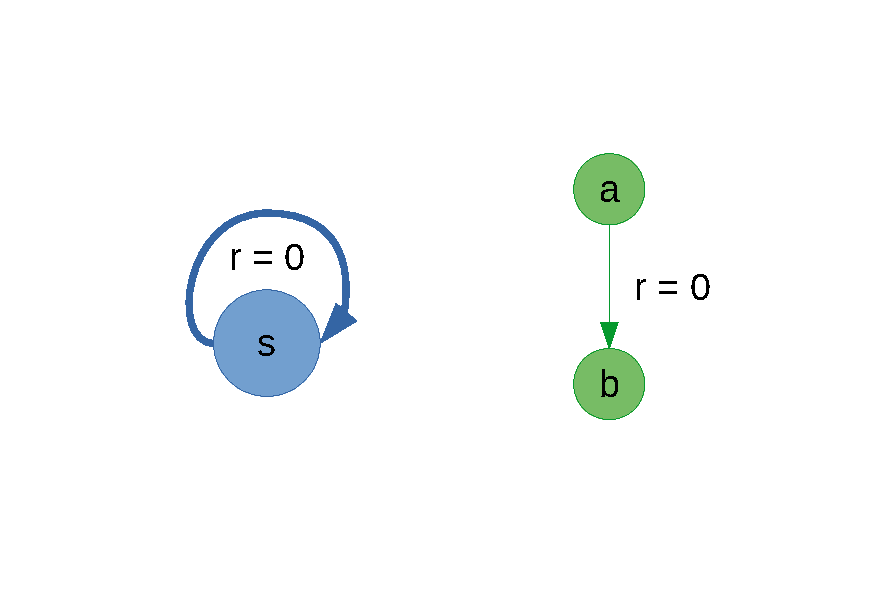
\includegraphics[trim=2cm 2cm 2cm 2cm, clip, width=0.4\textwidth]{img/simple_loop.pdf}\\
    \begin{tabular}{cccccc}
         \toprule
         Operator & $I$ & $\cB$ & $\cA\cB$ & $\cdots$ & $(\cA\cB)^k$ \\
         \midrule
         $U(a)$ & $V_{\max}$ & $\frac{1}{2} + \gamma V_{\max}$ & $\frac{1}{2} + \gamma V_{\max}$ && $\frac{1}{2}(1-\gamma^k)V_{\max} + \gamma^k V_{\max}$\\
         $U(b)$ & $V_{\max}$ & $V_{\max}$ & $\frac{1}{2} + \gamma V_{\max}$ && $\frac{1}{2}(1-\gamma^k)V_{\max} + \gamma^k V_{\max}$\\
         $L(a)$ & $0$ & $\frac{1}{2}$ & $\frac{1}{2}$ && $\frac{1}{2}(1-\gamma^k)V_{\max}$\\
		 $L(b)$ & $0$ & $0$ & $\frac{1}{2}$ && $\frac{1}{2}(1-\gamma^k)V_{\max}$\\
         \bottomrule
    \end{tabular}
    \caption{\textbf{Top}: a looping MDP with $|S|=|A|=1$, and the corresponding expanded tree $\Tau_1$ for a single observed transition. \textbf{Bottom}: the sequence of upper-bounds $(U_n)$ when alternating $A$ and $L$. We obtain $(U_k)$ and $(L_k)$ only go to their limit $V = \frac{1}{2}V_{\max}$ geometrically.}
    \label{fig:simple_loop}
\end{figure}

Alternatively, we can stop after a fixed number of iterations, e.g. $k=2$.

\subsection{Leaves pruning}
\label{sec:pruning}

Another observation can be made in the case where two nodes $a_1,a_2\in\Tau_n$ lead to the same state $s$:
\begin{proposition}[Pruning rule]
\label{prop:pruning}
Let $a_1,a_2\in\Tau_n$ such that state $s(a_1) = s(a_2) = s$ and $U = \cA(U) \geq V$ an aggregated upper-bound. 
\begin{equation}
\label{eq:pruning}
    \text{If } h(a_2) \geq h(a_1) \text{ and } U^a(a_2) \geq U^a(a_1)
    \text{, then }V(a_2) \geq V(a_1)
\end{equation}

In particular, there is no need to ever expand the node $a_1$.
\end{proposition}
\begin{proof}
Assume $h(a_2) \geq h(a_1)$.
\begin{align*}
    V(a_1) - V(a_2) &= R(a_1)- R(a_2) + \underbrace{\left(\gamma^{h(a_1)} - \gamma^{h(a_2)}\right)}_{\geq 0}V(s) \\
    &\leq R(a_1)- R(a_2) + \left(\gamma^{h(a_1)} - \gamma^{h(a_2)}\right)U(s)\\
    &= U^a(a_1) - U^a(a_2)
\end{align*}
Hence, if this last term is negative, then $V(a_1) - V(a_2)$ is as well.
\end{proof}

We propose that at each step, we detect such pairs $a_1, a_2$. Whenever $a_1$ is a leaf, we can remove it from the set $\cL_n^-\subset \cL_n $ of candidates for expansion.

\subsection{The algorithm}

\begin{algorithm}[H]
	\caption{State-aware planning}
	\label{alg:state-aware}
	\SetAlgoLined\DontPrintSemicolon
	\For{iteration $n$}{
		\nl Given $\Tau_n$, compute $L_n = (\cA_n\cB_n)^\infty(0)$ and $U_n = (\cA_n\cB_n)^\infty(V_{\max})$.\;
		\nl Select the optimistic sequence of actions $\hat{a}_{n}$ from \eqref{eq:sampling_rule}.\;
		\For(\tcp*[h]{Expand the corresponding leaf node}){action $a\in A$}{
			Add the child $\hat{a}_{n}a$ to the tree $\Gamma_{n+1}$ and observe its reward.
		}
		\nl Prune the tree: $\cL_{n+1}^- = \cP(\cL_{n+1})$.\;
	}
	\Return the recommendation $a_{n+1}$ from \eqref{eq:recommendation_rule}.\;
\end{algorithm}

\section{Regret bound}

In \autoref{thm:regret-bound-U}, we assumed that some bounds $L,U$ were revealed by and oracle and available from the onset for planning. In this section, we instead built a non-increasing (in the sense of inclusion) sequence of bounds $(L_n,U_n)_n\geq 0$, i.e. that verify $L_n\geq L_{n-1}\geq \dots\geq L_0\geq 0$ and $U_n\leq U_{n-1}\leq \dots\leq U_0\leq V_{\max}$.

We can consider the sequence $\kappa_n = \kappa(L_n, U_n)$. It is non-increasing and lower-bounded by $1$, thus converges to some $\kappa_\infty\in[1,K]$.
\begin{theorem}
The \autoref{alg:state-aware} enjoys the following regret bound: 
\begin{align*}
\forall \kappa'>\kappa_\infty, \quad r_n = \cO\left(n^{-\frac{\log 1/\gamma}{\log \kappa'}}\right)
\end{align*}
\end{theorem}

\begin{proof}
Let $\kappa'>\kappa_\infty$. Since $\kappa(L_n,U_n)\rightarrow\kappa_\infty$, there exists $n_0\in\Natural$ such that for all $n\geq n_0, \kappa(L_n,U_n) \leq \kappa'$.
We can show that at each iteration $n$, any expanded node must belong to $\Tau^\infty(L_n,U_n)$.
Let $n\geq n_0$, and define $d_0 = \min\{d\in\Natural: \exists t \in[n_0,n], \hat{a}_t\in A^d \}$. By definition, for all $d\geq d_0$, any expanded node of depth $d$ was expanded at a time $t\geq n_0$, and thus $\hat{a}_t\in\Tau^\infty_t \subset\Tau^\infty_{n_0}$. By denoting $n_d$ the number of expanded nodes of depth $d$, we obtain:
\[
n = \sum_{d=0}^{d_0-1}n_d + \sum_{d=d_0}^{d_n} n_d \leq  C_0 + C_1\sum_{d=d_0}^{d_n} (\kappa')^d \leq C_0 + C_1' (\kappa')^{d_n}
\]
And since $r_n \leq \frac{\gamma^{d_n}}{1-\gamma}$, we obtain the claimed bound.
\end{proof}

\section{Efficient implementation}

\paragraph{Time complexity}
 At each step, we perform a value iteration on $n$ nodes, which takes about $\cO\left(\frac{n K}{\log 1/\gamma}\right)$ steps. The entire planning procedure is $\cO\left(\frac{n^2 K}{\log 1/\gamma}\right)$.

In this section, we consider more efficient ways to implement the aggregation/backup and pruning rules described respectively in sections \ref{sec:aggregation} and \ref{sec:pruning}.

\paragraph{Aggregation and backup}
Let us denote $U^{(n)}$ the upper-bound used in the sampling rule \eqref{eq:sampling_rule} after $n$ leaf expansions, where $U^{(n)}$ is defined as the limit of \eqref{eq:recursion}. Assume that the previous iteration $n$, we stopped at some equilibrium $U^{(n)} = L(U^{(n)}) = A(U^{(n)})$.

At step $n+1$, after leaf expansion we obtain a novel tree $\Tau_{n+1}$. Instead of recomputing $U^{(n+1)}$ entirely from scratch using \eqref{eq:recursion}, we can instead initialise it with the previous value $U^{(n)}$ on $\Tau_n$ and $V_{\max}$ on the newly created leaves in $\Tau_{n+1} \setminus \Tau_n$.

We can notice that if we change the value of a single node $a$, the application of $L$ will only modify $U^{(n)}$ at its parents and leave the rest of the tree unchanged. Likewise, applying $A$ will only modify the values for the nodes in $\cN_n(a)$ and leave the rest of the tree unchanged. The idea of \autoref{algo:efficient} is

\paragraph{Leaves pruning}

When and how should we apply the rule \eqref{eq:pruning} described in \autoref{prop:pruning}?

The most straightforward way is to apply it once at every step, after the aggregations and backups.
The procedure needs to be applied within some equivalence classes $C(a)$ of nodes $a'$ that lead to the same state $s(a')=s(a)$. If a class $C$ is of size $n_C$, then the cost of running \eqref{eq:pruning} is $\cO(n_C^2)$. This could be improved to $\cO(n_C \log n_C)$ by computing the convex hull of the candidates points in $C$. Indeed, any point $a_1$ that does not belong to the top-frontier of this hull is dominated by some $a_2$, in the sense of \eqref{eq:pruning}.


\begin{algorithm}[htp]
  \SetAlgoLined\DontPrintSemicolon
  \SetKwFunction{expand}{expand}
  \SetKwFunction{update}{update}
  \SetKwFunction{backup}{backup}
  \SetKwProg{myalg}{Algorithm}{}{}
  \myalg{\expand{a}}{
  \For{action $b\in A$}{
  \nl Simulate action $b$ from state $s(a)$, observe reward $r$ and next state $s'$\;
  \nl Create a new node $ab$ with reward $r$,  state $s'$\;
  }
  \nl \update{a}\;
  \;
  }
  
  \setcounter{AlgoLine}{0}
  \SetKwProg{myproc}{Procedure}{}{}
  \myproc{\update{a}}{
  \uIf{$a$ is not a leaf}{
      \nl $U_{\text{backup}} \leftarrow \max_{b\in A} r(ab)+ \gamma U(s(ab))$\tcp*{Bellman backup $L$}
      \nl $\Delta \leftarrow U(s(a)) -  U_{\text{backup}}$\tcp*{Is the new bound tighter?}
      \nl \lIf{$\Delta > 0$}{$U(s(a))\leftarrow U_{\text{backup}}$\tcp*{Aggregation $A$}}
      \For{$a'\in\cN_n(a)$\tcp*{Recursion over updated nodes}}{
          \uIf{$a'$ is not the root and $\Delta > \epsilon(1-\gamma)\gamma^{-h(a)}$}{
              \nl \update{parent of $a'$}
          }
          }
  }
  }
  \caption{An recursive implementation of $(LA)^\infty$ with leaves pruning}
  \label{algo:efficient}
\end{algorithm} 

\section{Experiments}

\subsection{Full algorithm}

\subsubsection{Two-armed bandit}

We consider the simplest possible problem: 1 state and 2 actions, with rewards 0 and 1. The state-aware planner never expands a suboptimal node. In contrast, the tree expanded by \texttt{OPD} is quite balanced, even with such a dense reward and important gap.
\begin{figure}[H]
    \centering
    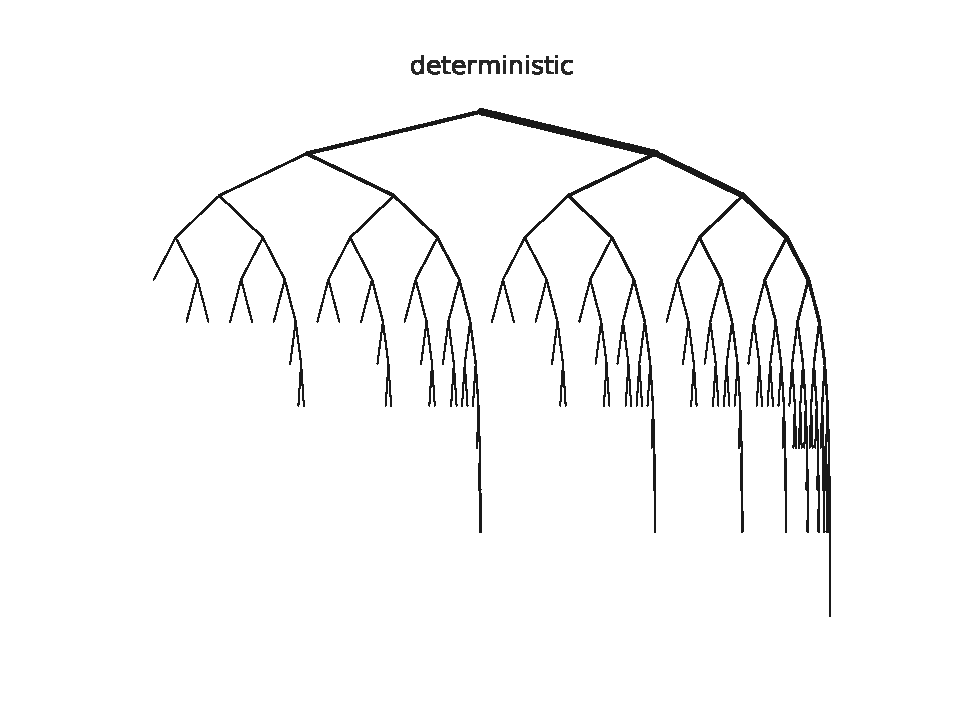
\includegraphics[width=0.49\textwidth]{img/bandit_deterministic.pdf}
    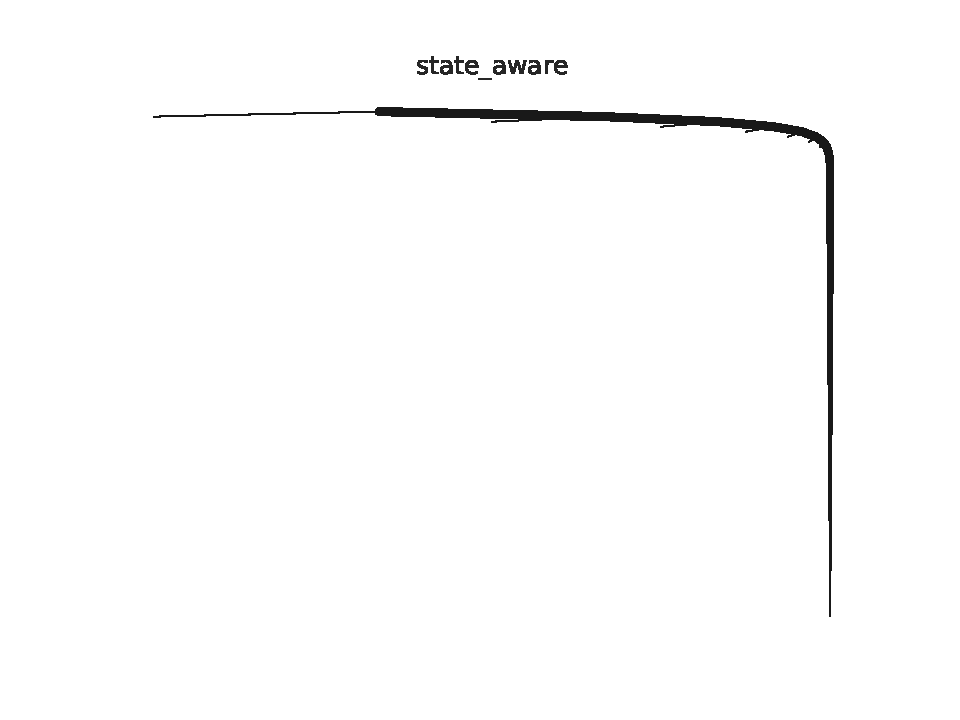
\includegraphics[width=0.49\textwidth]{img/bandit_state_aware.pdf}
    \caption{Trees expanded for $n = 200$, $\gamma=0.99$}
    \label{fig:bandit_trees}
\end{figure}

\subsubsection{Gridworld with 4 actions}

The reward is a paraboloid centred at $(10, 10)$ with length-scale of 5:  $r(x, y) = 1 - \frac{1}{5^2}((x-10)^2 + (y-10)^2)$ clipped to [0, 1].

\begin{figure}[H]
    \centering
    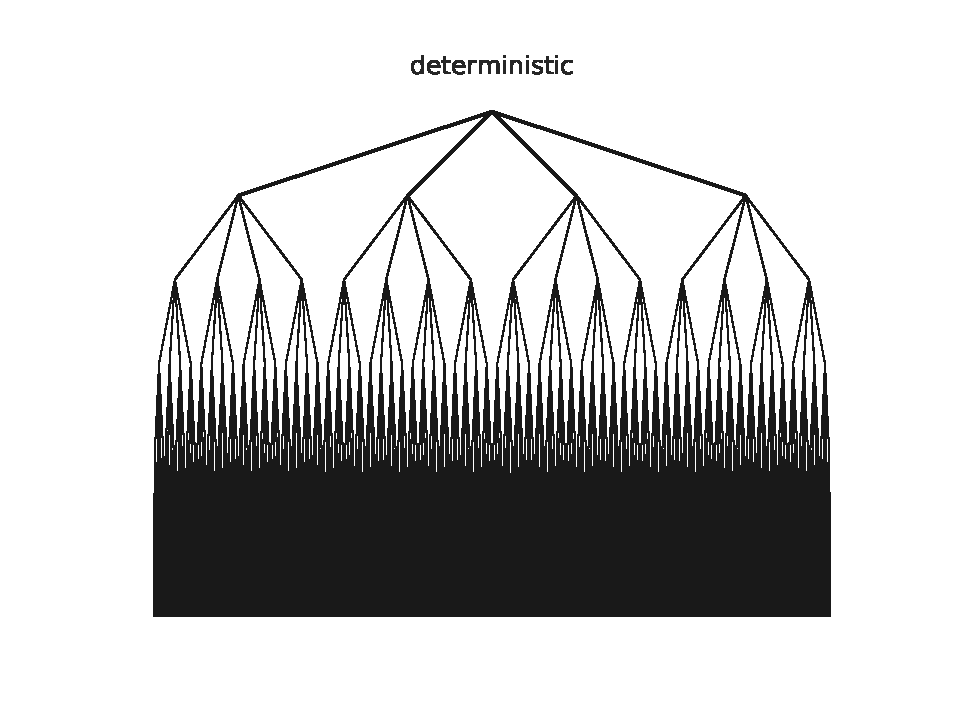
\includegraphics[width=0.49\textwidth]{img/4_deterministic.pdf}
    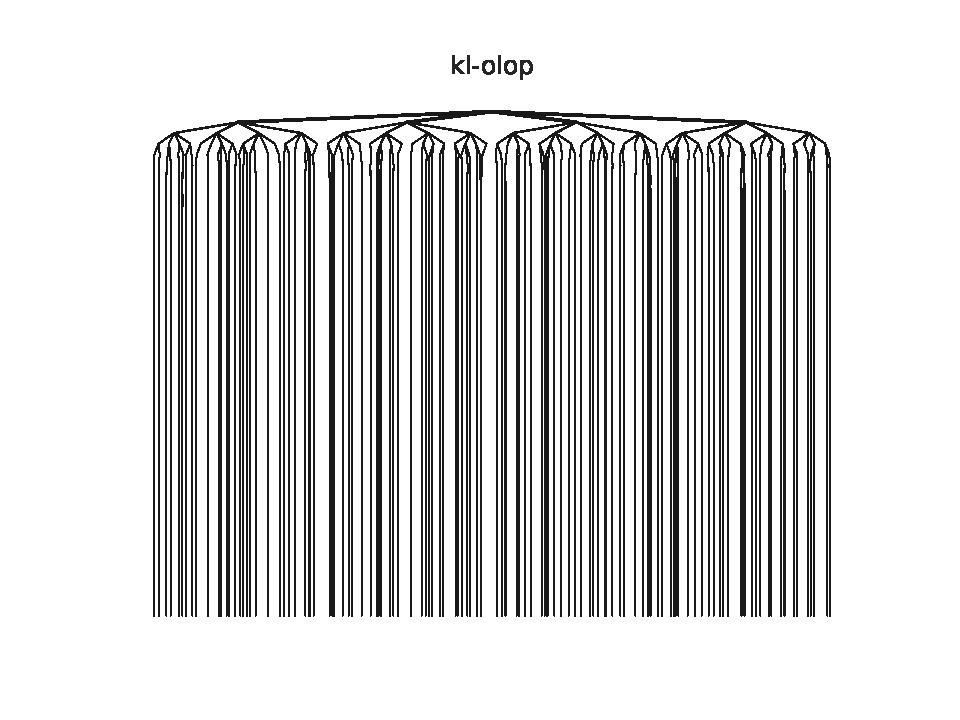
\includegraphics[width=0.49\textwidth]{img/4_kl-olop.pdf}
    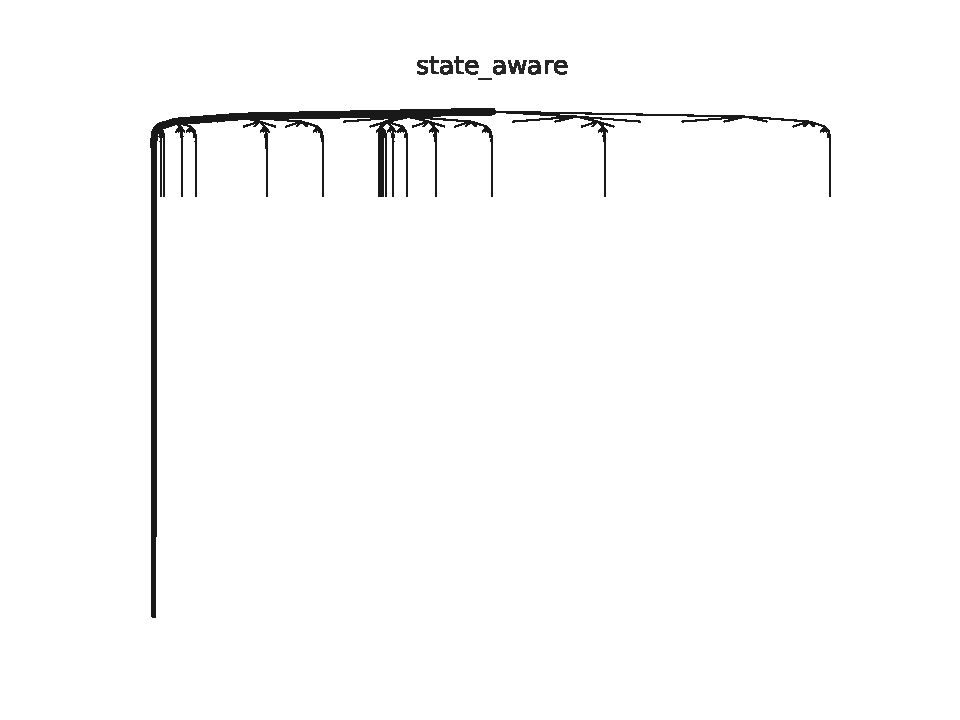
\includegraphics[width=0.49\textwidth]{img/4_state_aware.pdf}
    \caption{Trees expanded for $n = 5460$, $\gamma=0.95$}
    \label{fig:gw4_trees}
\end{figure}
\begin{figure}[H]
    \centering
    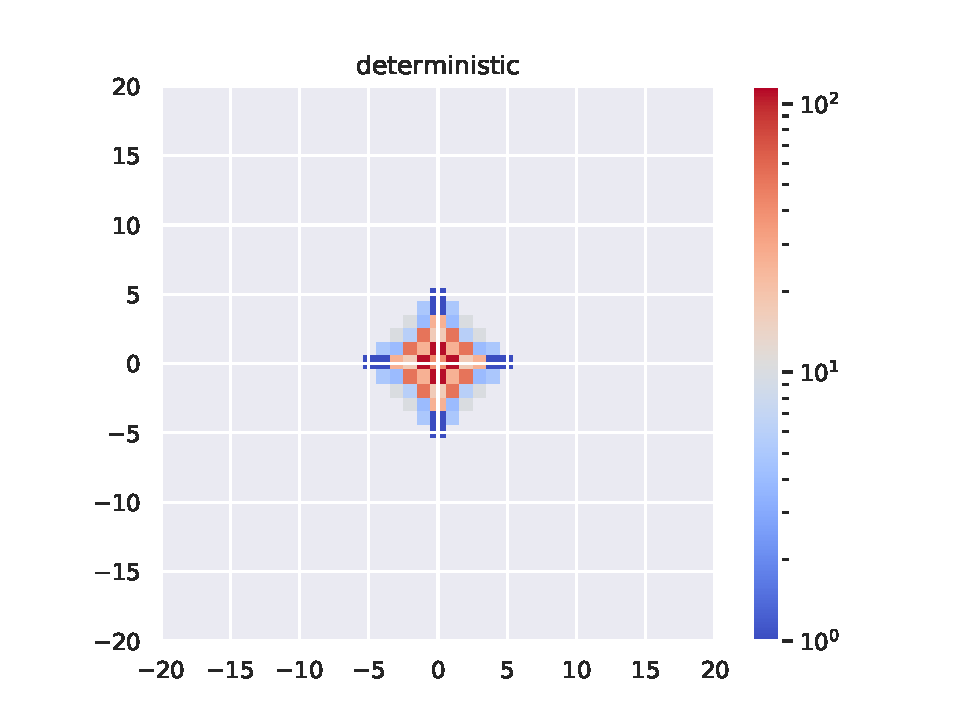
\includegraphics[width=0.49\textwidth]{img/4_occupations_deterministic.pdf}
    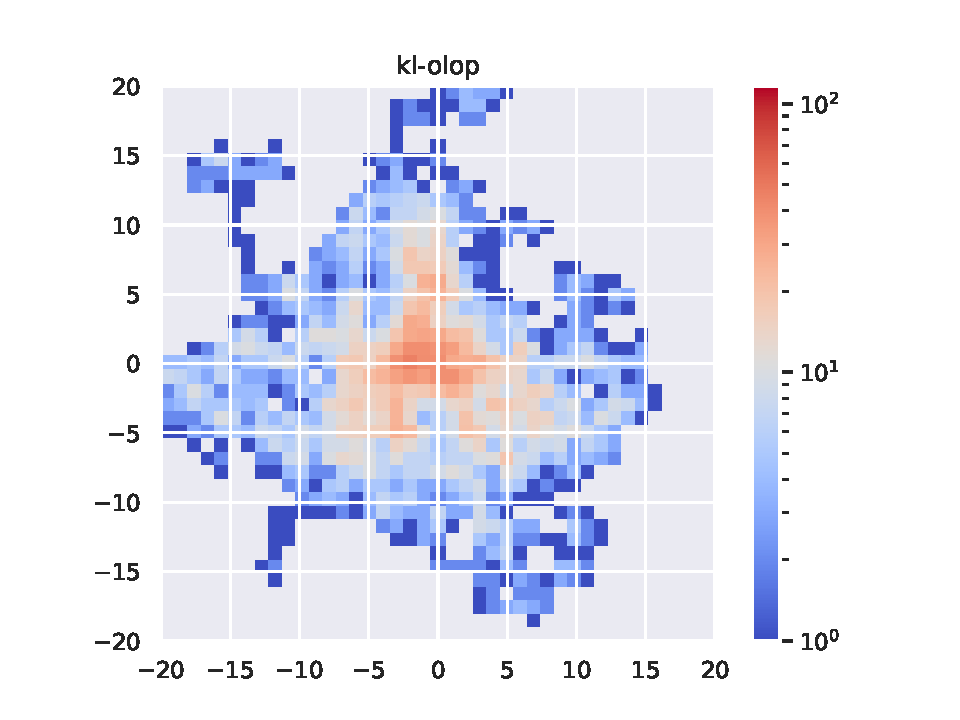
\includegraphics[width=0.49\textwidth]{img/4_occupations_kl-olop.pdf}
    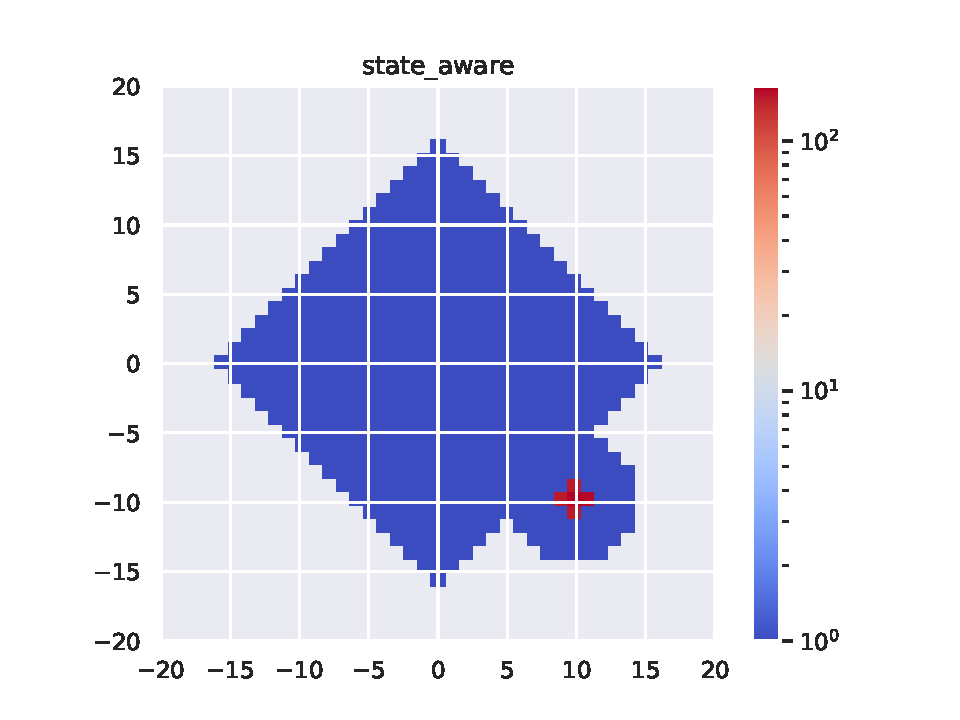
\includegraphics[width=0.49\textwidth]{img/4_occupations_state_aware.pdf}
    \caption{Number of visits for $n = 5460$, $\gamma=0.95$}
    \label{fig:gw4_visits}
\end{figure}
\begin{figure}[H]
    \centering
    % \includegraphics[width=0.49\textwidth]{img/4_updates_deterministic.pdf}
    % \includegraphics[width=0.49\textwidth]{img/4_updates_kl-olop.pdf}
    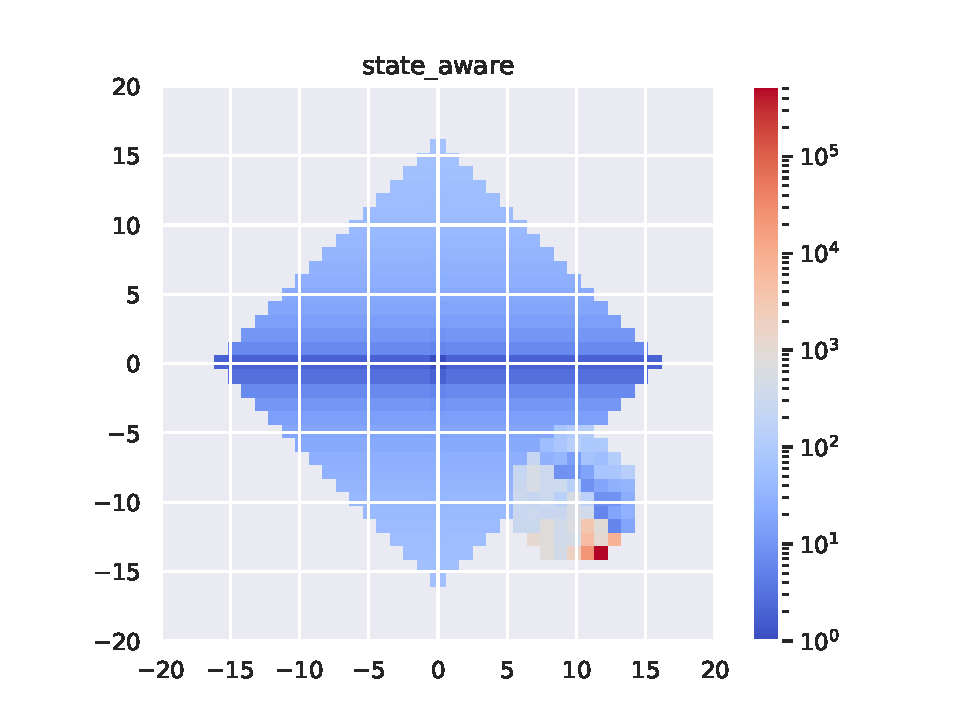
\includegraphics[width=0.49\textwidth]{img/4_updates_state_aware.pdf}
    \caption{Number of updates in the leaf expansion for $n = 5460$, $\gamma=0.95$}
    \label{fig:gw4_updates}
\end{figure}

% \subsubsection{Gridworld with 8 actions}

% We add the diagonal actions.

% \begin{figure}[H]
%     \centering
%     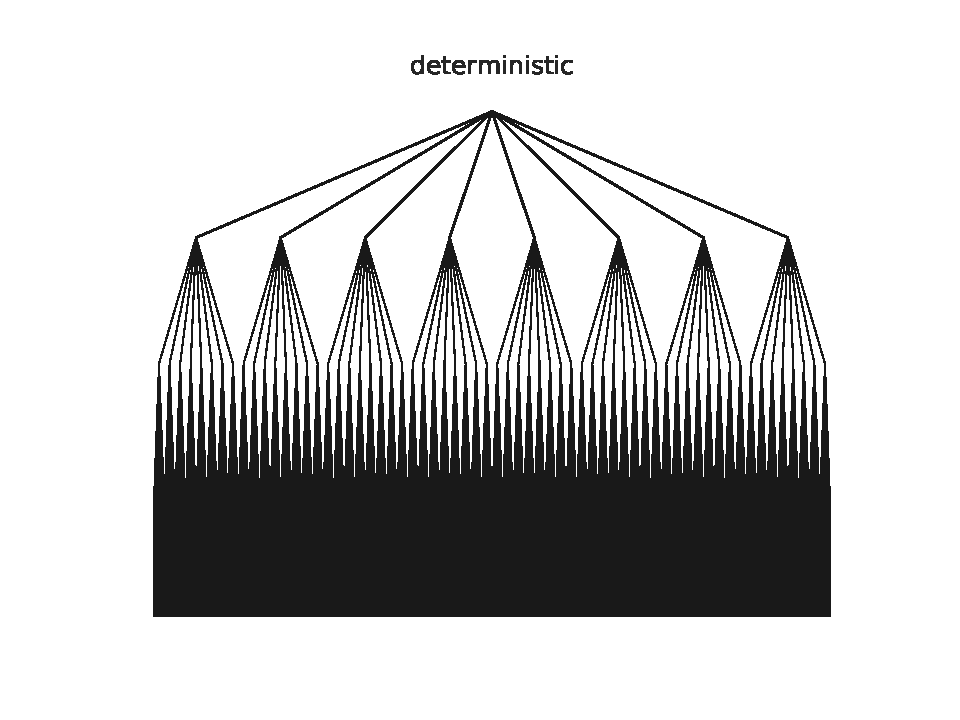
\includegraphics[width=0.49\textwidth]{img/8_deterministic.pdf}
%     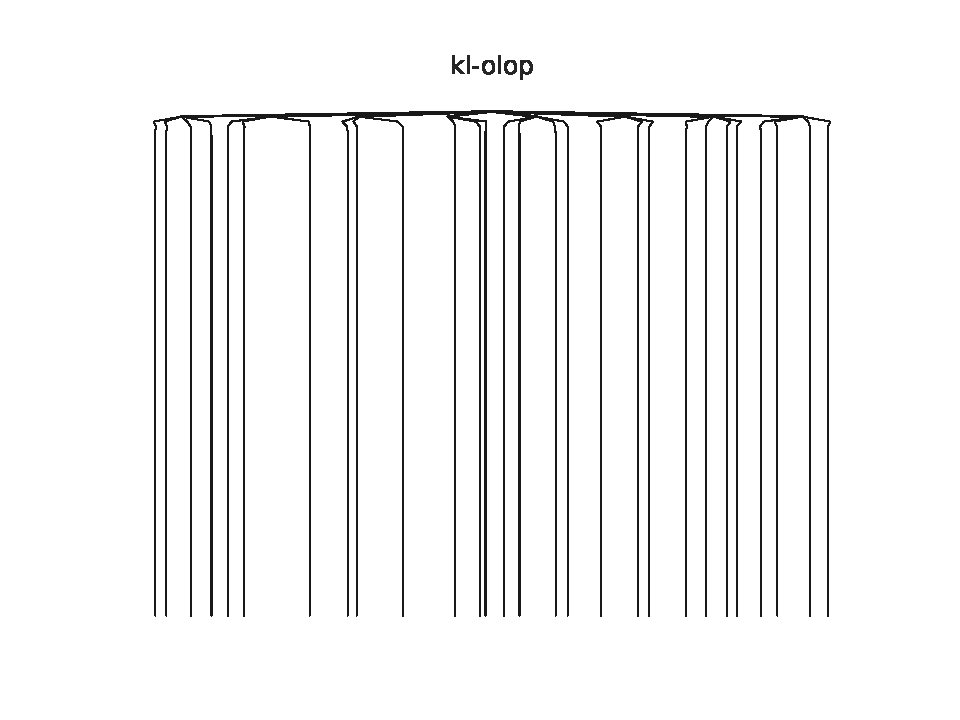
\includegraphics[width=0.49\textwidth]{img/8_kl-olop.pdf}
%     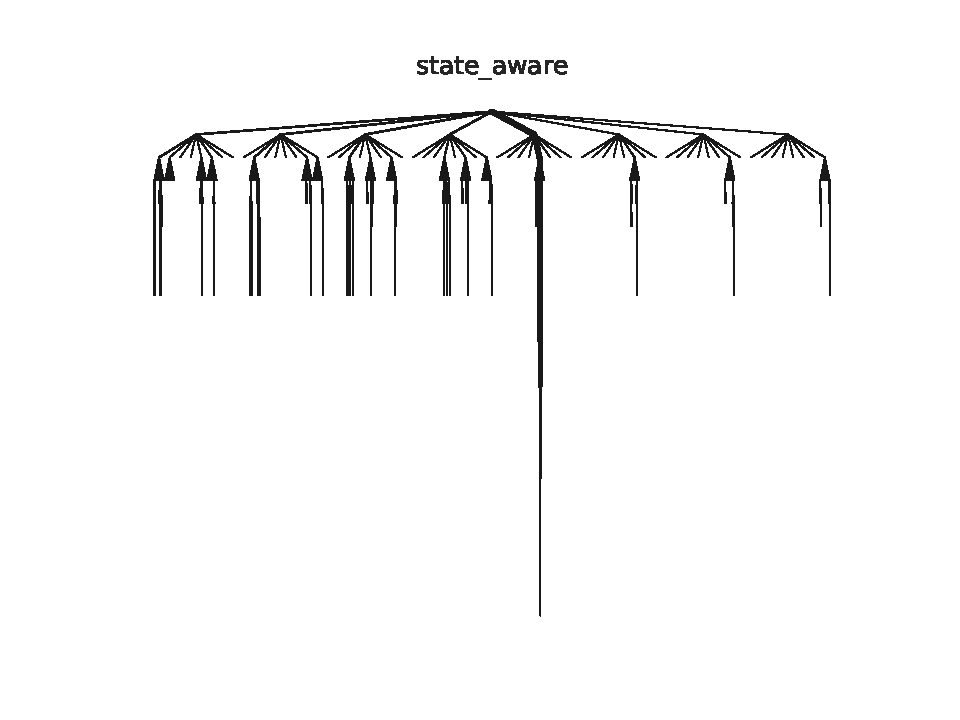
\includegraphics[width=0.49\textwidth]{img/8_state_aware.pdf}
%     \caption{Trees expanded for $n = 4680$, $\gamma=0.95$}
%     \label{fig:my_label}
% \end{figure}
% \begin{figure}[H]
%     \centering
%     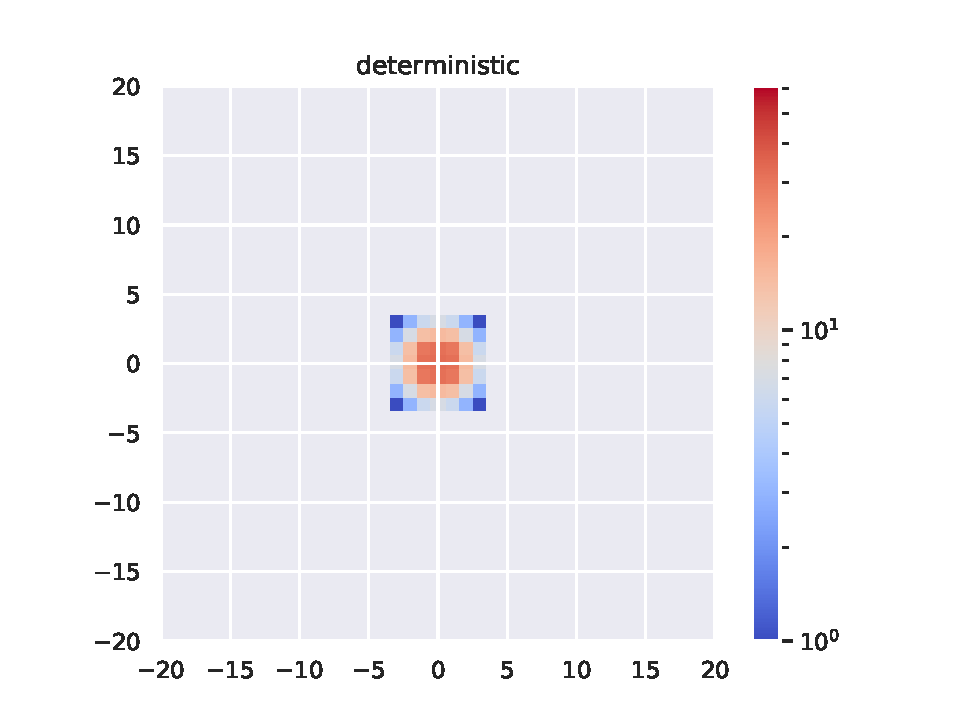
\includegraphics[width=0.49\textwidth]{img/8_states_deterministic.pdf}
%     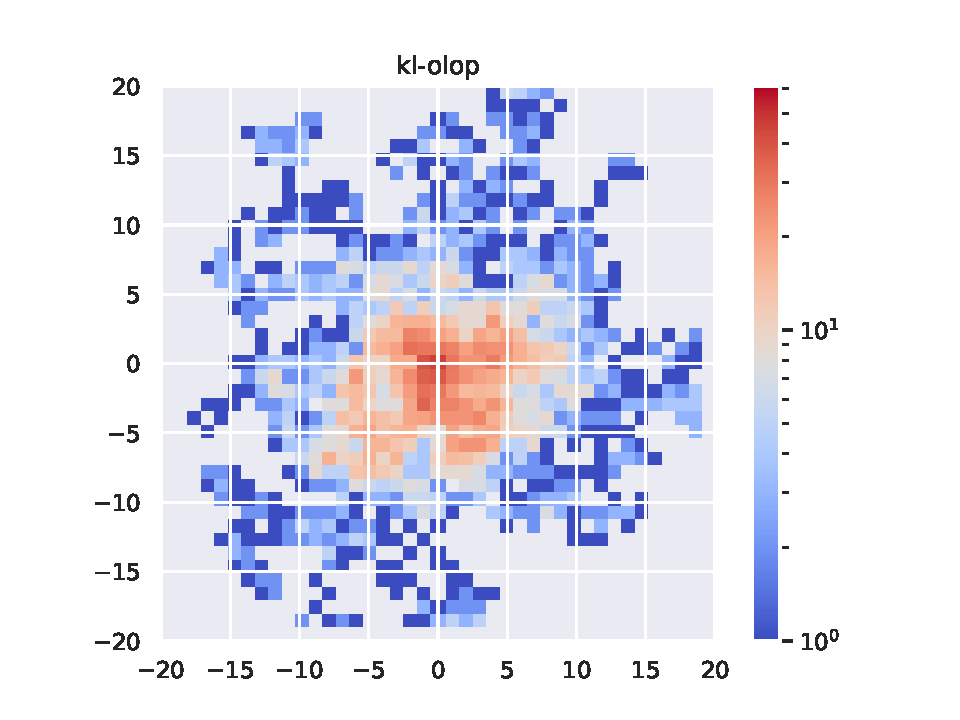
\includegraphics[width=0.49\textwidth]{img/8_states_kl-olop.pdf}
%     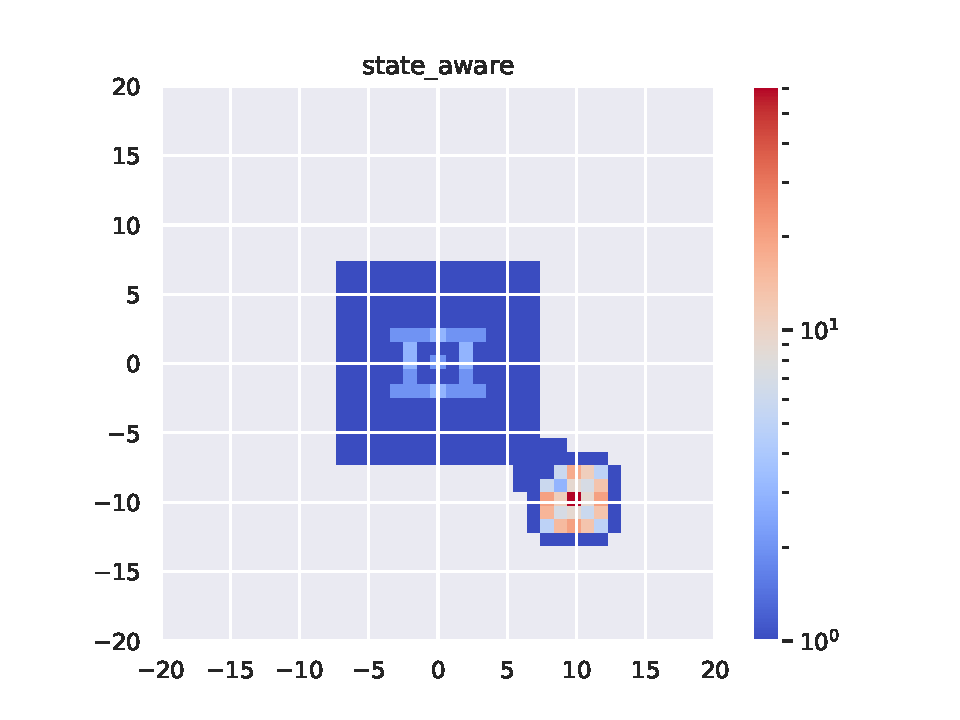
\includegraphics[width=0.49\textwidth]{img/8_states_state_aware.pdf}
%     \caption{Trees expanded for $n = 4680$, $\gamma=0.95$}
%     \label{fig:my_label}
% \end{figure}

\subsection{Effect of the early stopping}

\begin{figure}[H]
    \centering
    \begin{subfigure}[b]{\textwidth}
        \centering
        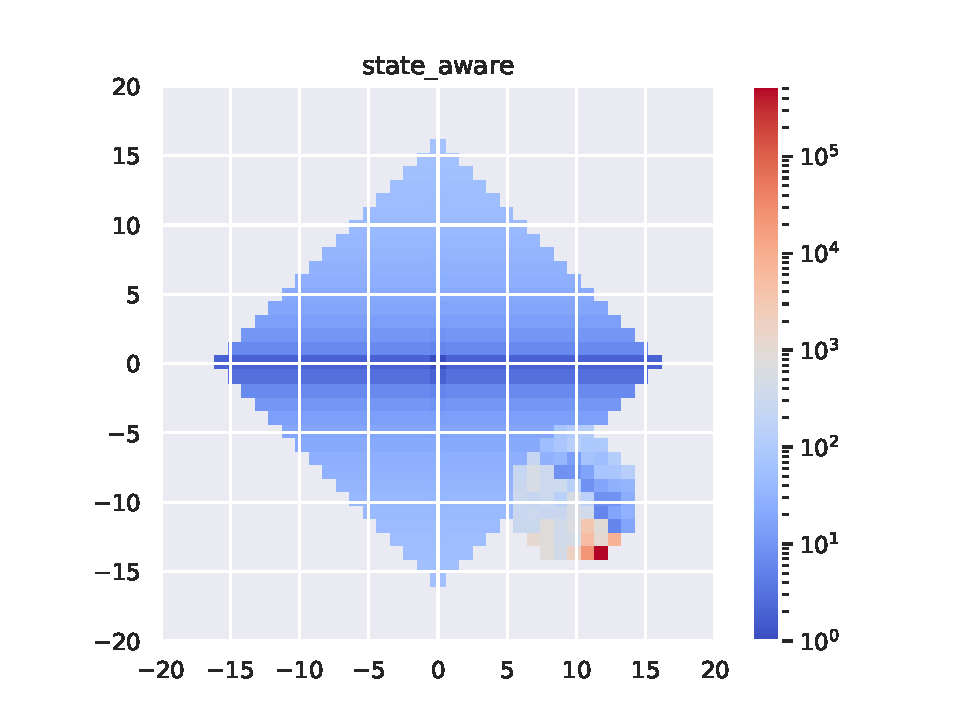
\includegraphics[width=0.49\linewidth]{img/epsilon/0/updates_state_aware.pdf}
        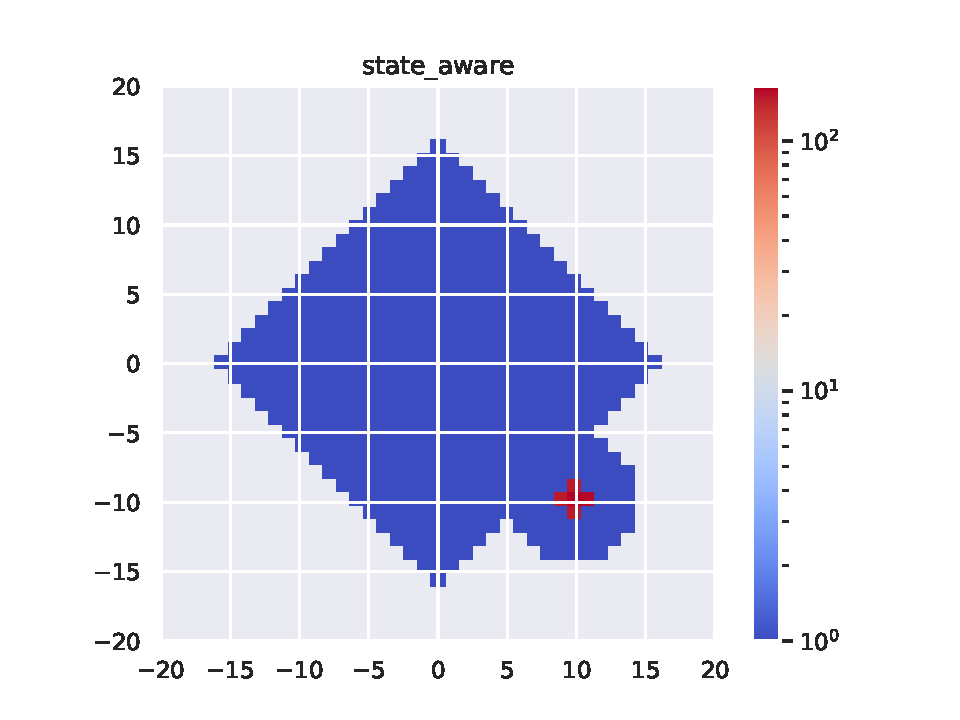
\includegraphics[width=0.49\linewidth]{img/epsilon/0/occupations_state_aware.pdf}
        \caption{$\epsilon=0$}
    \end{subfigure}
    \begin{subfigure}[b]{\textwidth}
        \centering
        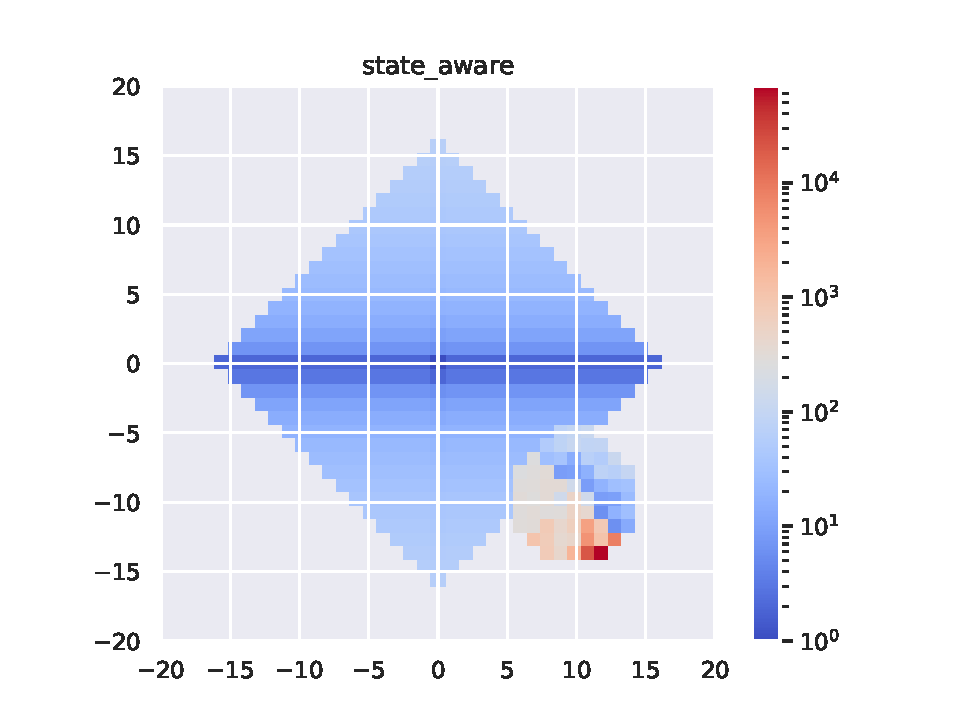
\includegraphics[width=0.49\textwidth]{img/epsilon/1e-2/updates_state_aware.pdf}
        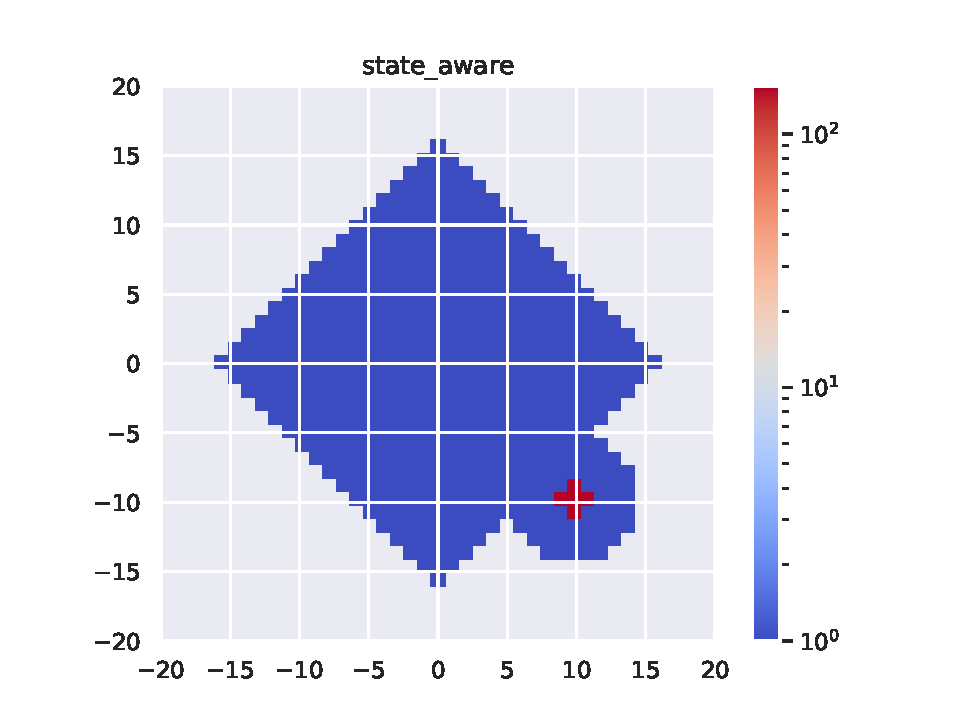
\includegraphics[width=0.49\textwidth]{img/epsilon/1e-2/occupations_state_aware.pdf}
        \caption{$\epsilon=1e-2$}
    \end{subfigure}
    \begin{subfigure}[b]{\textwidth}
        \centering
        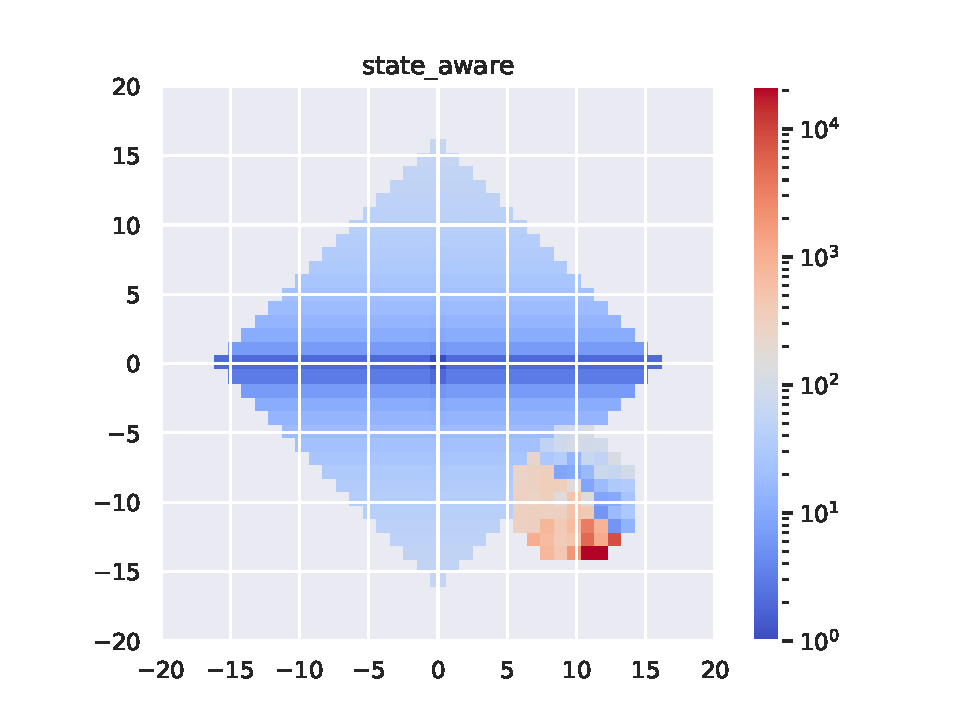
\includegraphics[width=0.49\textwidth]{img/epsilon/1e-1/updates_state_aware.pdf}
        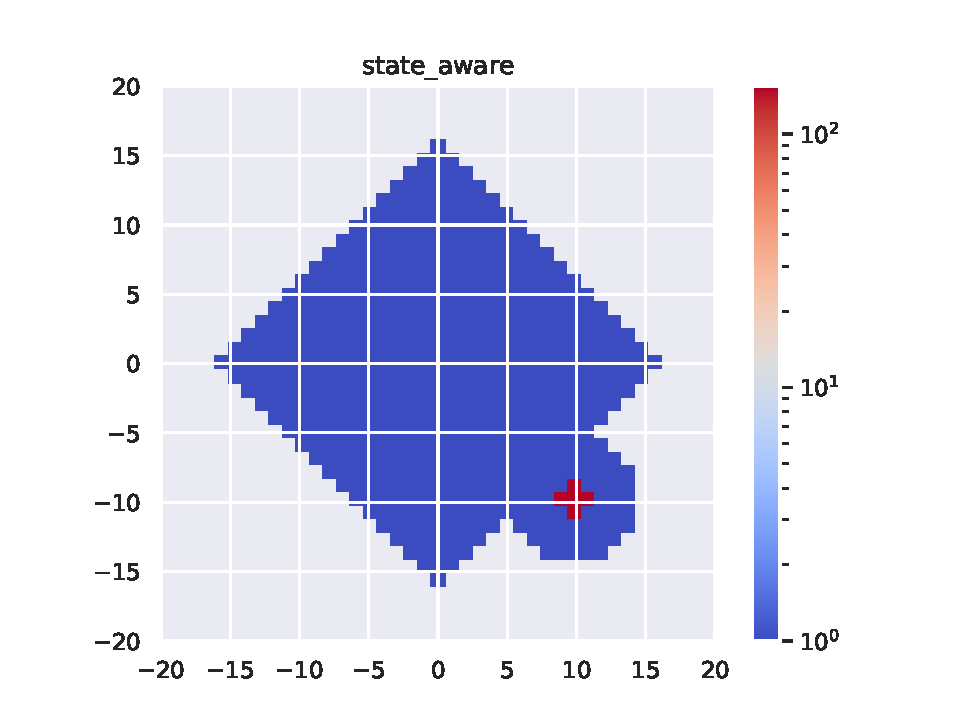
\includegraphics[width=0.49\textwidth]{img/epsilon/1e-2/occupations_state_aware.pdf}
        \caption{$\epsilon=1e-1$}
    \end{subfigure}
    \caption{Updates and occupancies for various values of $\epsilon$, for $n = 5460$, $\gamma=0.95$}
    \label{fig:epsilon_1}
\end{figure}
\begin{figure}[H]
\ContinuedFloat
    \centering
    \begin{subfigure}[b]{\textwidth}
        \centering
        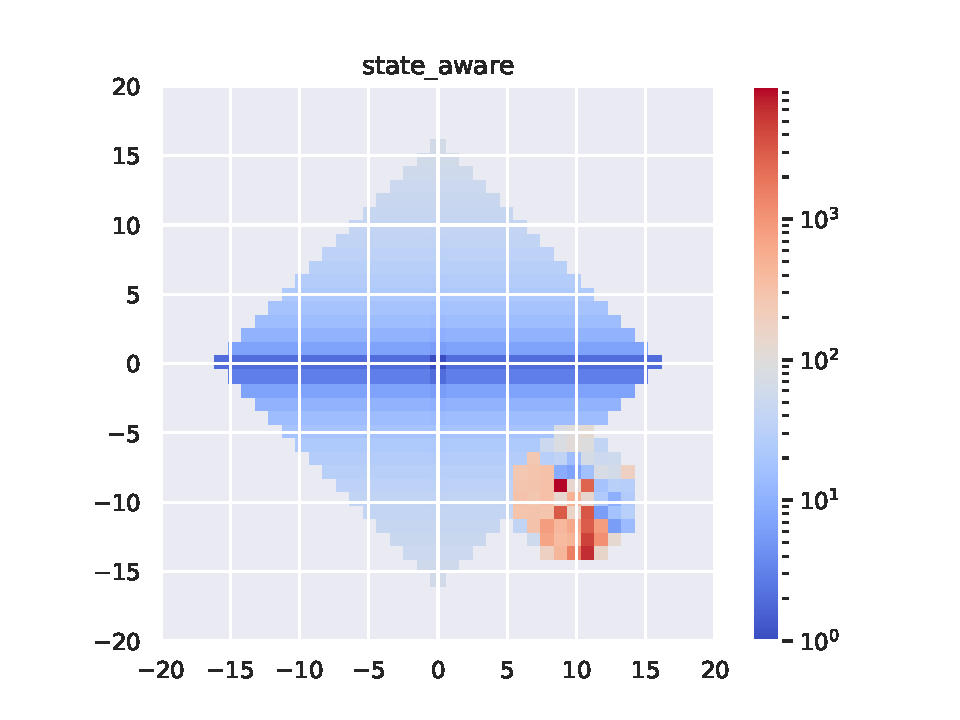
\includegraphics[width=0.49\textwidth]{img/epsilon/1e0/updates_state_aware.pdf}
        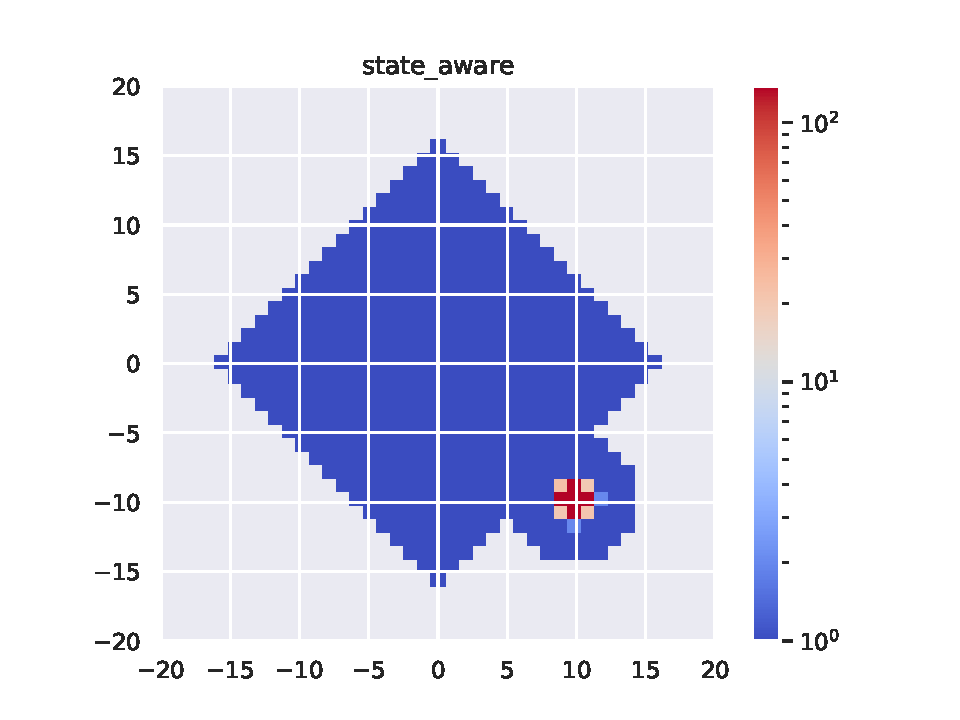
\includegraphics[width=0.49\textwidth]{img/epsilon/1e0/occupations_state_aware.pdf}
        \caption{$\epsilon=1e0$}
    \end{subfigure}
    \begin{subfigure}[b]{\textwidth}
        \centering
        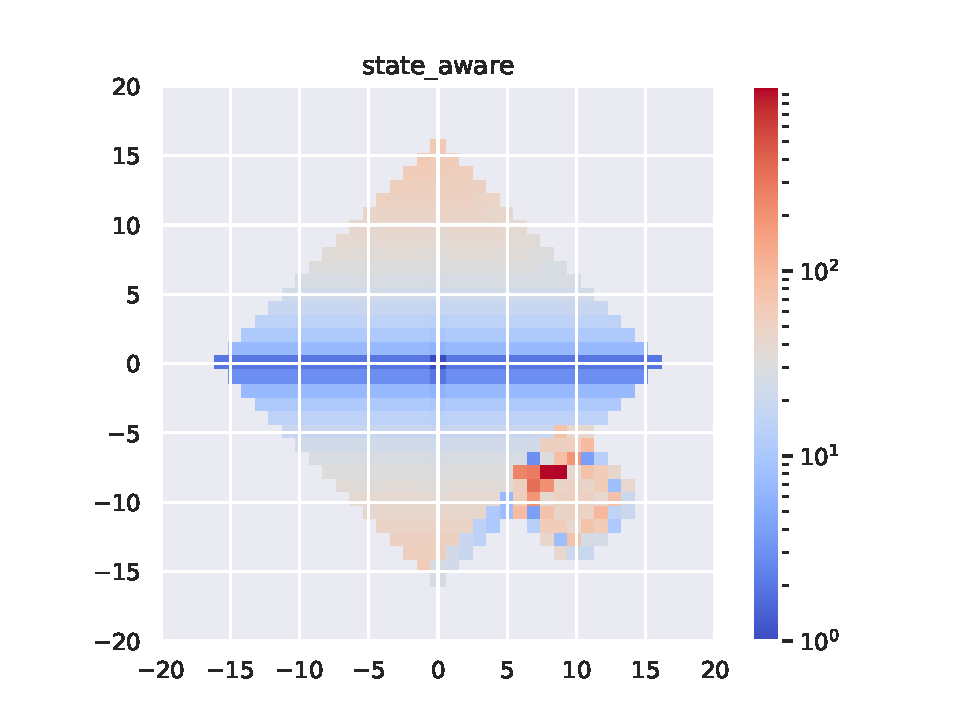
\includegraphics[width=0.49\textwidth]{img/epsilon/1e1/updates_state_aware.pdf}
        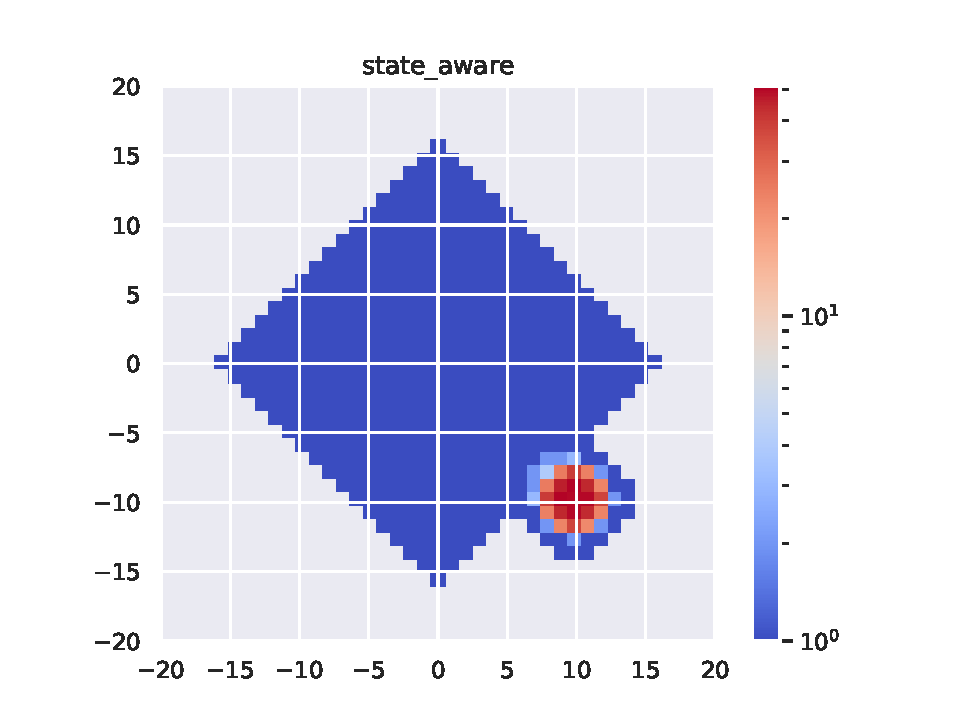
\includegraphics[width=0.49\textwidth]{img/epsilon/1e1/occupations_state_aware.pdf}
        \caption{$\epsilon=1e1$}
    \end{subfigure}
    \begin{subfigure}[b]{\textwidth}
        \centering
        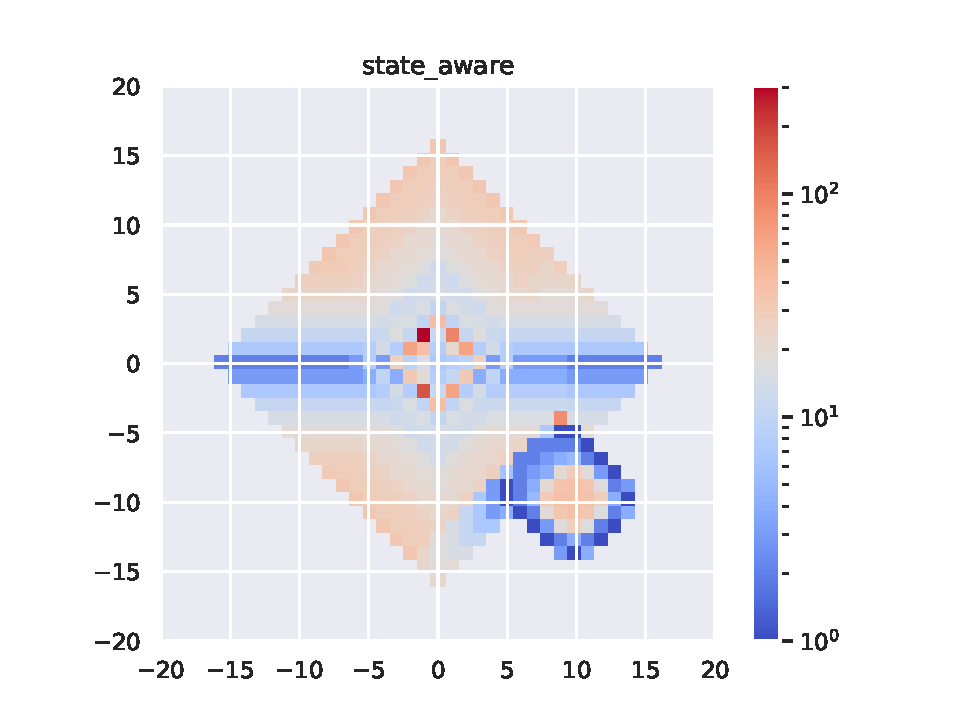
\includegraphics[width=0.49\textwidth]{img/epsilon/1e2/updates_state_aware.pdf}
        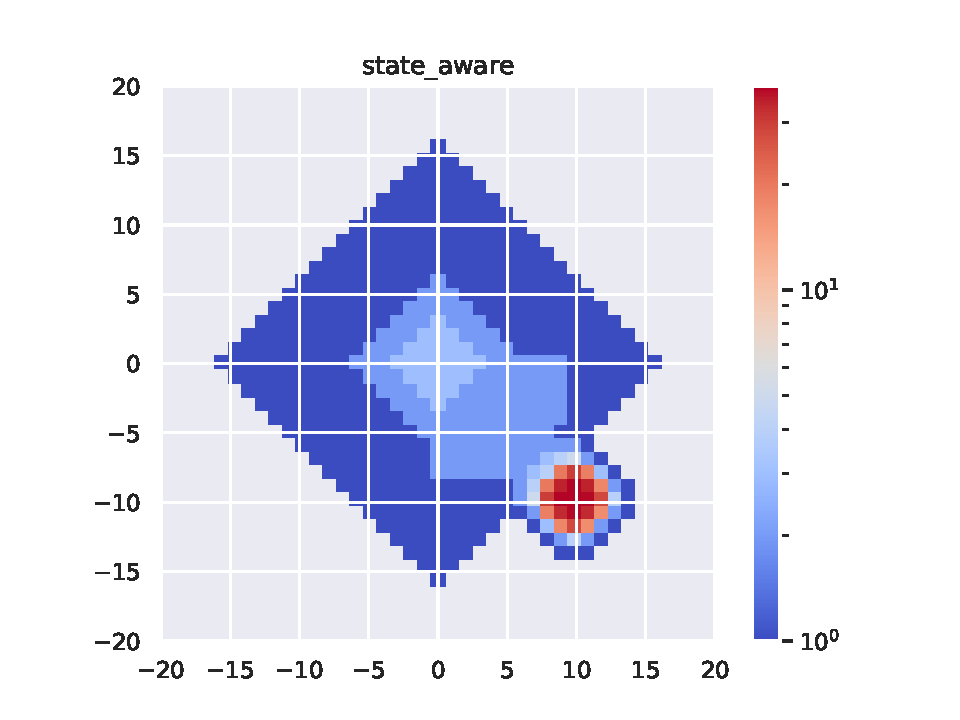
\includegraphics[width=0.49\textwidth]{img/epsilon/1e2/occupations_state_aware.pdf}
        \caption{$\epsilon=1e2 = V_{\max}$}
    \end{subfigure}
    \caption{Updates and occupancies for various values of $\epsilon$, for $n = 5460$, $\gamma=0.95$}
\end{figure}

\end{document}
